\section{Infraestructura Cloud y Análisis de Costes}
\label{sec:infraestructura}

Uno de los pilares de este trabajo es la demostración de la viabilidad económica del proyecto mediante el uso de infraestructura cloud optimizada.

\subsection{Ecosistema AWS: ECS y ECR}
Para el despliegue y orquestación del modelo, se ha seleccionado Amazon Web Services (AWS), aprovechando los siguientes servicios:
\begin{itemize}
    \item \textbf{Amazon Elastic Container Registry (ECR):} Actúa como el repositorio privado de imágenes de Docker, integrado totalmente con el flujo de CI/CD de GitHub Actions.
    \item \textbf{Amazon Elastic Container Service (ECS):} Se utiliza para la orquestación de los contenedores. A diferencia de un despliegue en instancias EC2 puras, ECS facilita la gestión del ciclo de vida de la aplicación, el escalado y el autorreparado de tareas.
\end{itemize}

\subsection{Estrategia de Spot Instances}
El coste es el principal inhibidor en el desarrollo de modelos de lenguaje. Para mitigar esto, el clúster de ECS se ha configurado para utilizar \textbf{Amazon EC2 Spot Instances}. Estas instancias permiten acceder a la capacidad computacional sobrante de AWS con descuentos de hasta el 90\% sobre el precio de las instancias bajo demanda. 

\subsubsection{Identificación y Etiquetado}
Siguiendo las buenas prácticas de gestión de infraestructura, cada instancia se identifica mediante etiquetas (*tags*). Se ha definido el nombre \texttt{nexus-slm} (asignado a la clave \texttt{Name}) como estándar para permitir un seguimiento sencillo de los recursos activos en la consola de AWS y mediante scripts de automatización.

\begin{figure}[H]
    \centering
    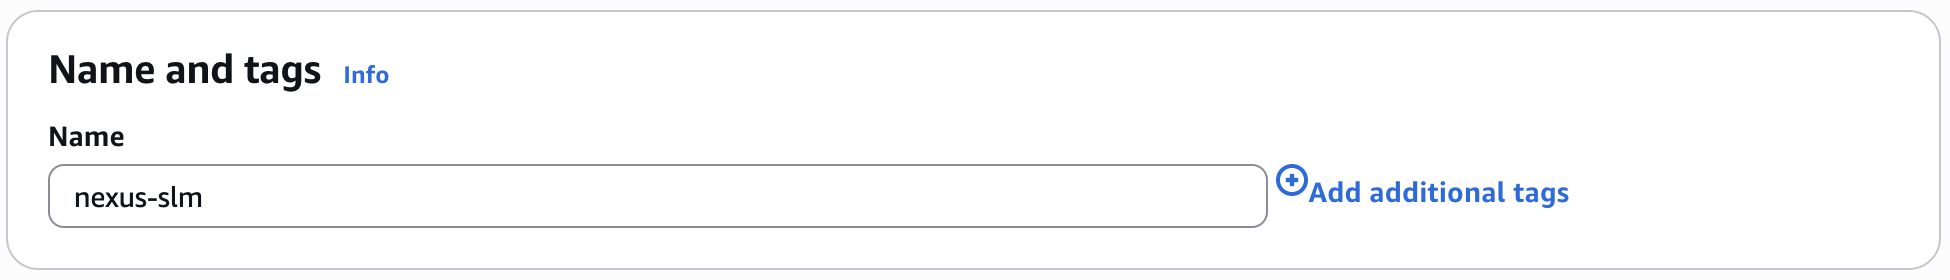
\includegraphics[width=0.8\textwidth]{images/aws_infrastructure/instance_name.png}
    \caption{Configuración del nombre de la instancia en la consola de AWS.}
    \label{fig:aws_instance_name}
\end{figure}

\subsubsection{Selección de la Imagen de Máquina (AMI)}
Para que el software sea capaz de comunicarse eficientemente con el hardware de aceleración, es crítico seleccionar una \textit{Amazon Machine Image} (AMI) que proporcione el entorno base adecuado.

Se ha seleccionado la AMI: \textbf{Deep Learning Base AMI with Single CUDA (Amazon Linux 2023)}. Esta imagen viene preconfigurada con los \textit{drivers} de NVIDIA y el \textit{toolkit} de CUDA necesarios para el entrenamiento del modelo, eliminando la complejidad técnica de la instalación manual y garantizando la compatibilidad entre el kernel de Linux y los núcleos Tensor de la GPU.

\begin{figure}[H]
    \centering
    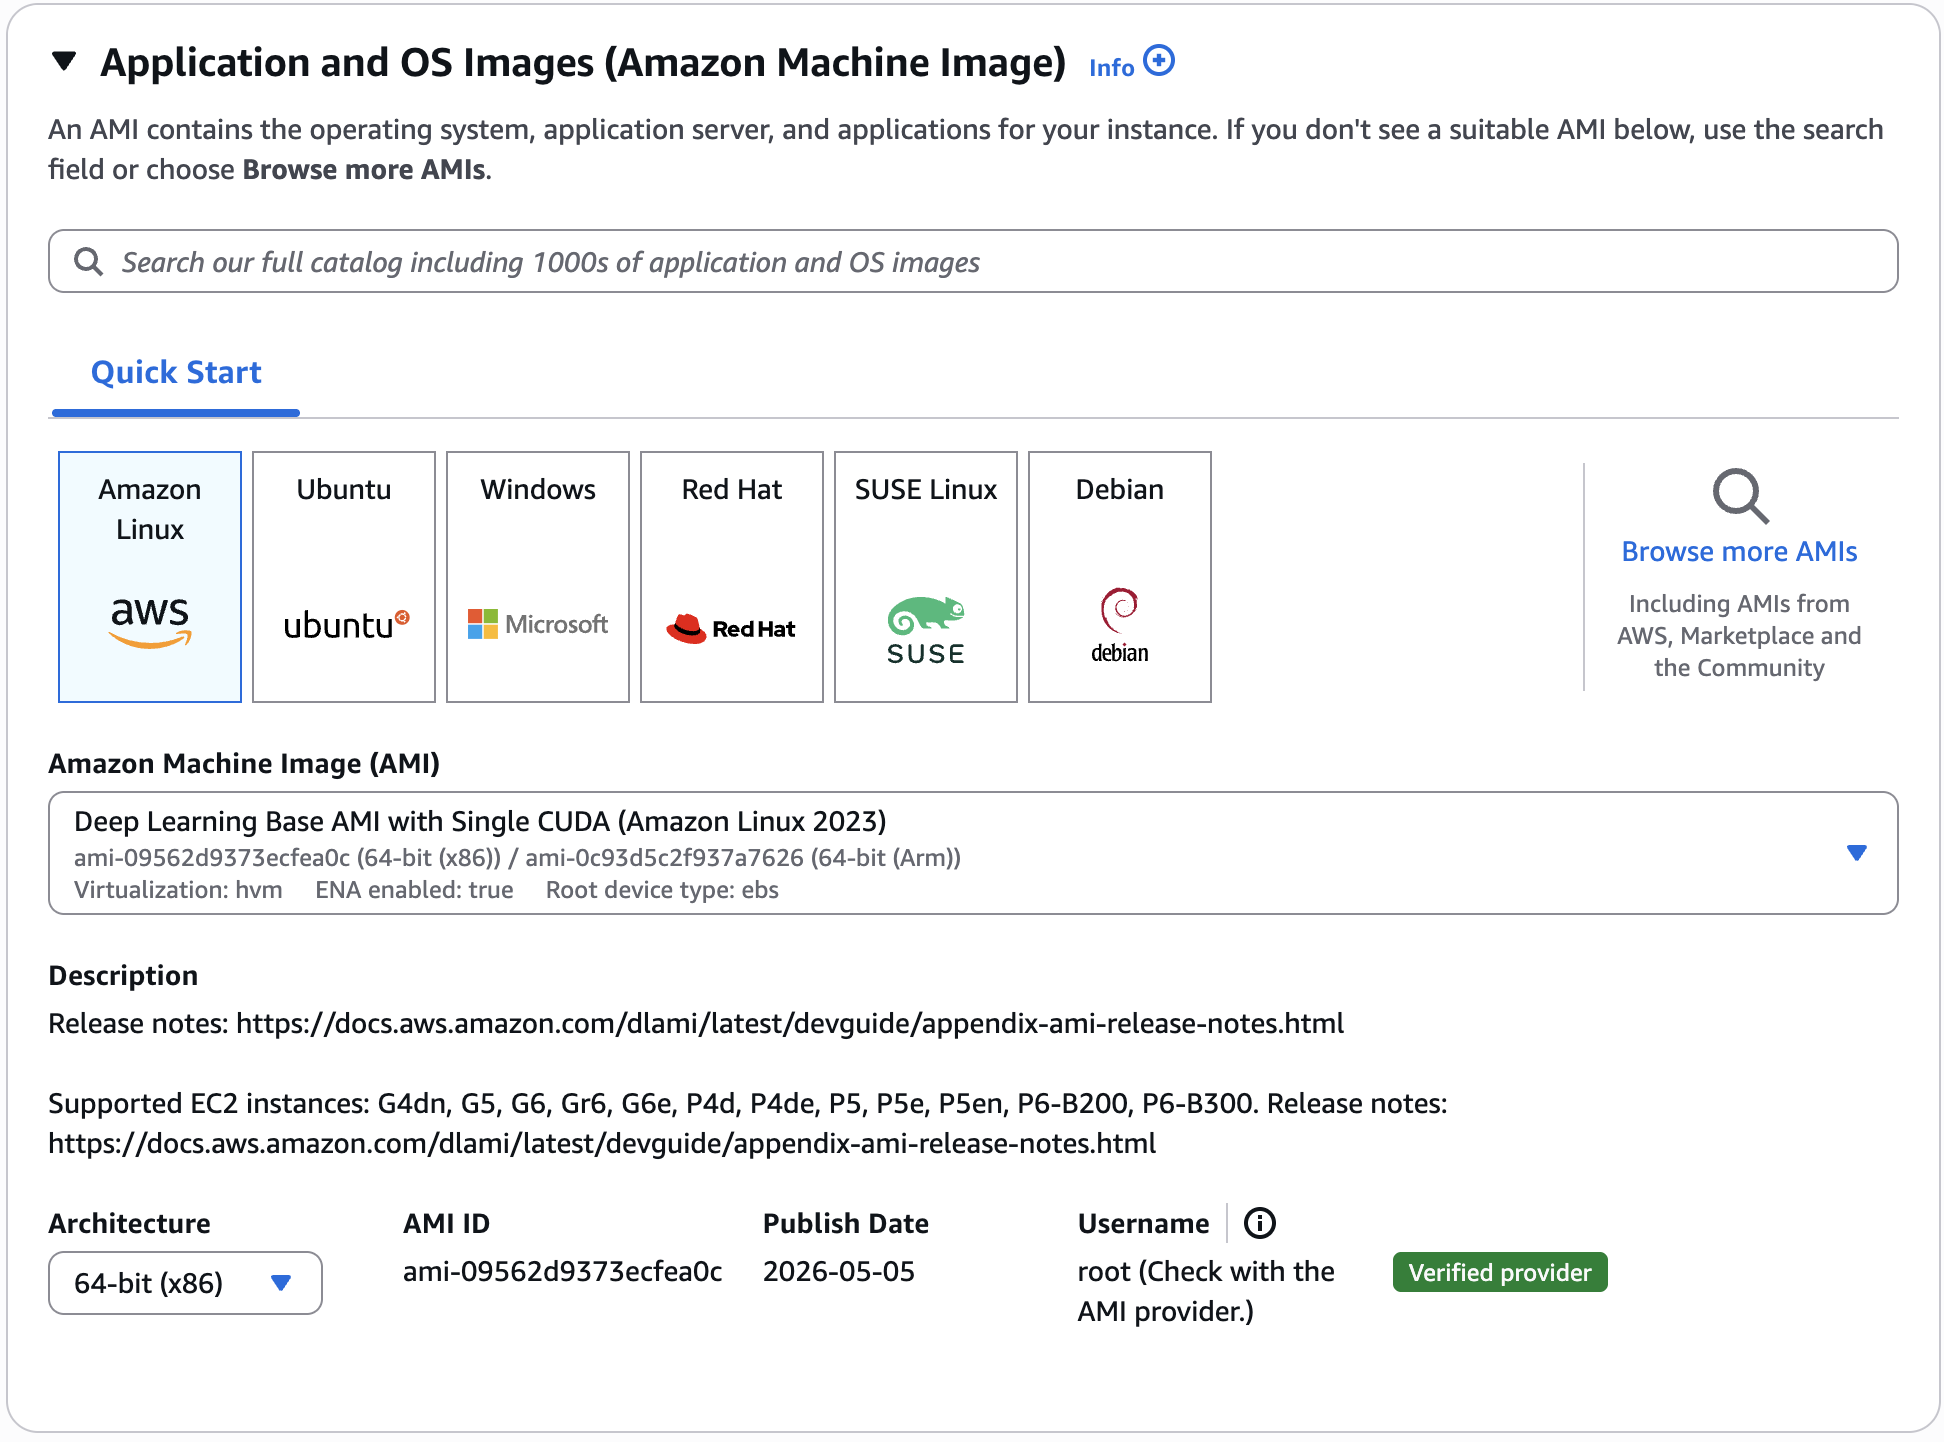
\includegraphics[width=0.8\textwidth]{images/aws_infrastructure/AMI.png}
    \caption{Interfaz de selección de la AMI especializada para Deep Learning con soporte CUDA.}
    \label{fig:aws_ami}
\end{figure}

Esta elección habilita el uso de una amplia gama de instancias optimizadas para computación acelerada. A continuación, se detallan las familias de instancias compatibles y sus especificaciones de hardware:

\begin{table}[H]
\centering
\begin{tabularx}{\textwidth}{|l|X|l|}
\hline
\textbf{Instancia} & \textbf{Hardware GPU} & \textbf{Propósito Principal} \\ \hline
\texttt{G4dn} & NVIDIA T4 (16 GB VRAM) & Inferencia y entrenamiento ligero \\ \hline
\texttt{G5} & NVIDIA A10G (24 GB VRAM) & Entrenamiento de modelos SLM / Gráficos \\ \hline
\texttt{G6 / Gr6} & NVIDIA L4 (24 GB VRAM) & Eficiencia energética y IA generativa \\ \hline
\texttt{G6e} & NVIDIA L40S (48 GB VRAM) & LLMs de tamaño medio y LLM Fine-tuning \\ \hline
\texttt{P4d / P4de} & NVIDIA A100 (40/80 GB VRAM) & Cómputo de alto rendimiento (HPC) \\ \hline
\texttt{P5 / P5e / P5en} & NVIDIA H100 (80 GB VRAM) & Entrenamiento de modelos de lenguaje masivos \\ \hline
\texttt{P6-B200 / B300} & NVIDIA Blackwell & Próxima generación de IA de ultra-escala \\ \hline
\end{tabularx}
\caption{Familias de instancias EC2 soportadas por la AMI de Deep Learning y su hardware asociado.}
\label{tab:aws_instances}
\end{table}

\subsubsection{Selección del Hardware: Tipo de Instancia}
Tras definir el entorno de software, el siguiente paso crítico es la elección del hardware subyacente. El tipo de instancia de EC2 determina la capacidad de CPU, memoria ram, almacenamiento y rendimiento de red del host que ejecutará el modelo.

Para este proyecto, se ha seleccionado la familia de instancias \textbf{G6}. Esta elección se fundamenta en la necesidad de disponer de una gran capacidad de memoria de video (VRAM) y un ancho de banda de memoria elevado, factores indispensables para almacenar y procesar los pesos de la arquitectura Transformer y los estados ocultos de la GRU durante el entrenamiento.

Consultando las especificaciones técnicas oficiales de AWS, observamos que la familia G6 ofrece diversas configuraciones escalables basadas en procesadores AMD EPYC 7R13 y aceleradores NVIDIA L4:

\begin{figure}[H]
    \centering
    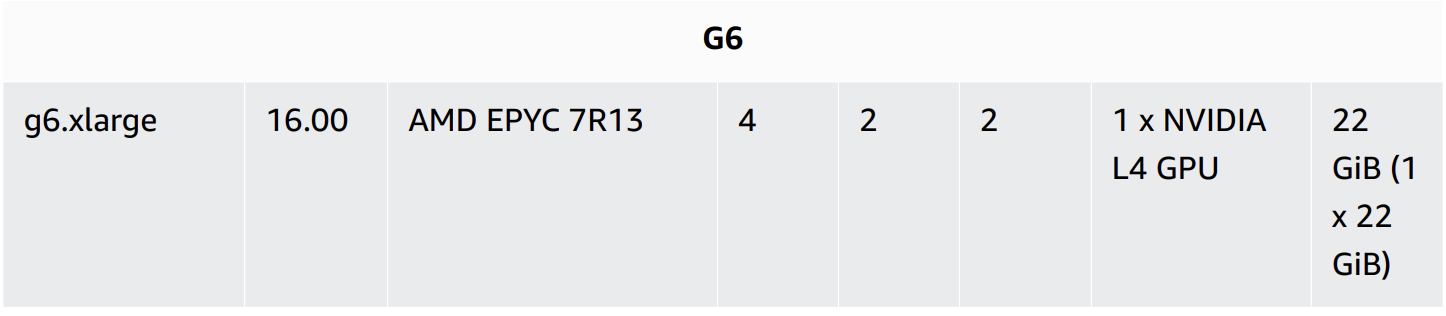
\includegraphics[width=0.9\textwidth]{images/aws_infrastructure/G6_instance_0.png}
    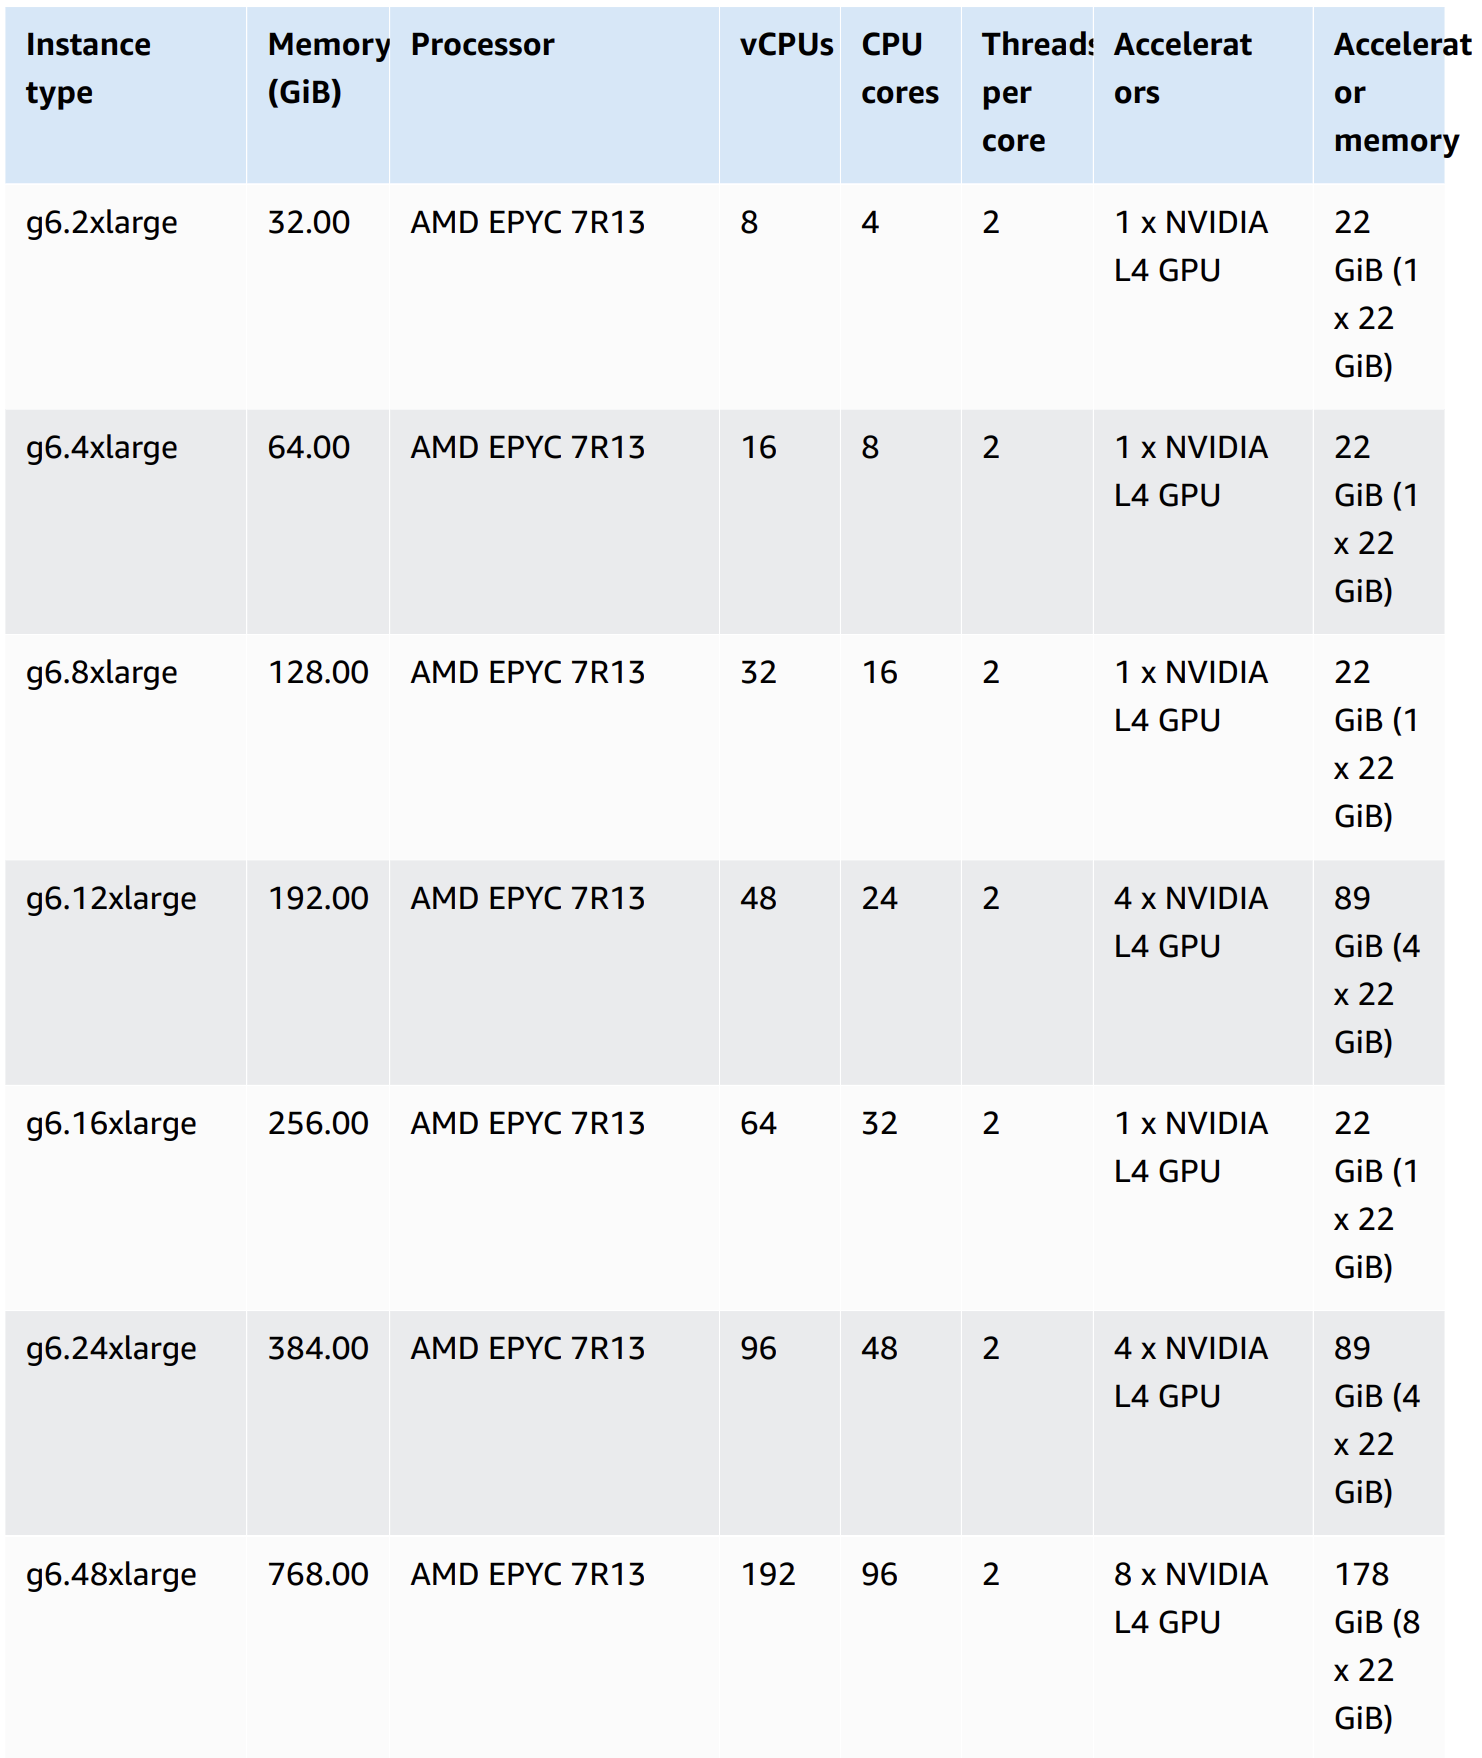
\includegraphics[width=0.9\textwidth]{images/aws_infrastructure/G6_instance_1.png}
    \caption{Especificaciones de hardware para las diferentes variantes de la familia de instancias G6.}
    \label{fig:aws_g6_specs}
\end{figure}

La versatilidad de la serie G6 permite desde configuraciones económicas con una sola GPU (como la \texttt{g6.xlarge} con 22 GB de VRAM) hasta potentes nodos de cómputo con múltiples aceleradores, proporcionando el equilibrio ideal entre coste y rendimiento para un Small Language Model.

\subsubsection{Configuración Técnica y Automatización}
Para garantizar la estabilidad del entrenamiento bajo el modelo de subasta de Spot, se han implementado las siguientes configuraciones técnicas adicionales:
\begin{itemize}
    \item \textbf{Launch Templates:} Definición de plantillas de lanzamiento que especifican las familias detalladas anteriormente, permitiendo que el clúster elija dinámicamente según disponibilidad.
    \item \textbf{Capacity Providers:} Gestión del escalado automático de las instancias de infraestructura.
    \item \textbf{Gestión de Interrupciones:} Señales de terminación de 2 minutos para realizar el guardado automático (\textit{checkpointing}) en Amazon S3.
\end{itemize}

Esta estrategia es ideal para las fases de entrenamiento y fine-tuning del SLM, donde la tolerancia a interrupciones es gestionada mediante la capacidad de ECS para relanzar tareas automáticamente en nuevas instancias disponibles.

\subsection{Evaluación de Rendimiento vs Coste}
Presentación de gráficas y métricas que comparan el tiempo de ejecución con el gasto económico real, demostrando la eficiencia de la arquitectura híbrida en entornos de recursos limitados.
